\documentclass[12pt, letterpaper]{article}
\usepackage[T1,T2A]{fontenc}
\usepackage[russian]{babel}
\usepackage[utf8]{inputenc}
\usepackage{amsmath}
\DeclareMathOperator\erf{erf}
\usepackage{listings}
\usepackage{xcolor, graphicx}
\usepackage{float}
\usepackage{tikz}
\usepackage{hyperref}
\usepackage{pgfplots}
\pgfplotsset{compat=1.16}
\hypersetup{
    colorlinks=true,
    linkcolor=cyan,
    filecolor=magenta,      
    urlcolor=blue,
    pdfpagemode=FullScreen,
    }
\title{Отчёт по лабораторной работе №22 по курсу “Алгоритмы и структуры данных”}
\author{Цирулев Николай}
\begin{document}
\maketitle
\begin{description}
\textbf{Студент группы:} \underline{М80-108Б-22 Цирулев Николай Владимирович, № по списку 21}\\
\textbf{Контакты e-mail:} \underline{mrcirniko@gmail.com}\\
\textbf{Работа выполнена:} \underline{«26» марта 2023 г.}\\
\textbf{Преподаватель:} \underline{асп. каф. 806 Сахарин Никита Александрович}\\
\textbf{Входной контроль знаний с оценкой:}\\
\textbf{Отчет сдан} \underline{«1» апреля 2023 г.,}\\ \textbf{итоговая оценка}\\
\textbf{Подпись преподавателя:} \underline{\hspace{3cm}}\\
\end{description}
\section{Тема}
\textbf{Издательская система \TeX}
\section{Цель работы}
\textbf{Получить навыки работы с документами в издательской системе \LaTeX}
\section{Задание}
\textbf{Оформить отсчет по лабораторной работе в издательской системе \LaTeX}
\section{Оборудование}
\textit {Процессор:} AMD Ryzen 5 5500U with Radeon Graphics 2.10 GHz\\
\textit{ОП:} 16GB\\
\textit {SSD:} 220GB
\section{Программное обеспечение}
\textbf{Операционная система семейства} UNIX, \textbf{наименование} Ubuntu, \textbf{версия} 20.04 LTS \textbf{Интерпретатор команд} bash, версия 5.0.11(1)-release \textbf{Редактор текстов} nano, \textbf{версия} 4.8
\section{Идея, метод, алгоритм решения}
Продемонстрируем самые используемые функции \LaTeX.
\section{Сценарий выполнения работы}
\subsection{Пример формул}

$x^{2}+y^{2}=R^2$\\
\\
$\frac{sin(x)}{cos(x)}=tg(x)$\\
\\
$\sum^n_{i=1}a_i+\sum^m_{j=n+1}a_j=\sum^m_{i=1}a_i$\\
\\
$sin(\varphi)=\sqrt{1-cos(\varphi)^2}$\\
\subsection{Пример графики}
\begin{figure}[H]
    \centering
    \begin{tikzpicture}
        \begin{axis}[
            xlabel=$x$,
            ylabel=$y$,
            zlabel={$f(x,y) = \sin(x)\cos(y)$},
            domain=-2*pi:2*pi,
            y domain=-2*pi:2*pi,
            samples=20,
            view={45}{30},
            width=0.8\textwidth,
            height=0.6\textwidth,
        ]
            \addplot3[surf] {sin(deg(x))*cos(deg(y))};
        \end{axis}
    \end{tikzpicture}
    \caption{3D график функции $f(x,y) = \sin(x)\cos(y)$}
\end{figure}
\begin{figure}[H]
    \begin{tikzpicture}
        \draw[->] (-3,0) -- (3,0) node[right] {$x$};
        \draw[->] (0,-1) -- (0,5) node[above] {$y$};
        \draw[scale=1,domain=-2:2,smooth,variable=\x,blue] plot ({\x},{\x*\x}) node[right] {$f(x)=x^2$};
    \end{tikzpicture}
    \caption{2D график функции $f(x)=x^2$}
\end{figure}


\begin{figure}[H]
\centering
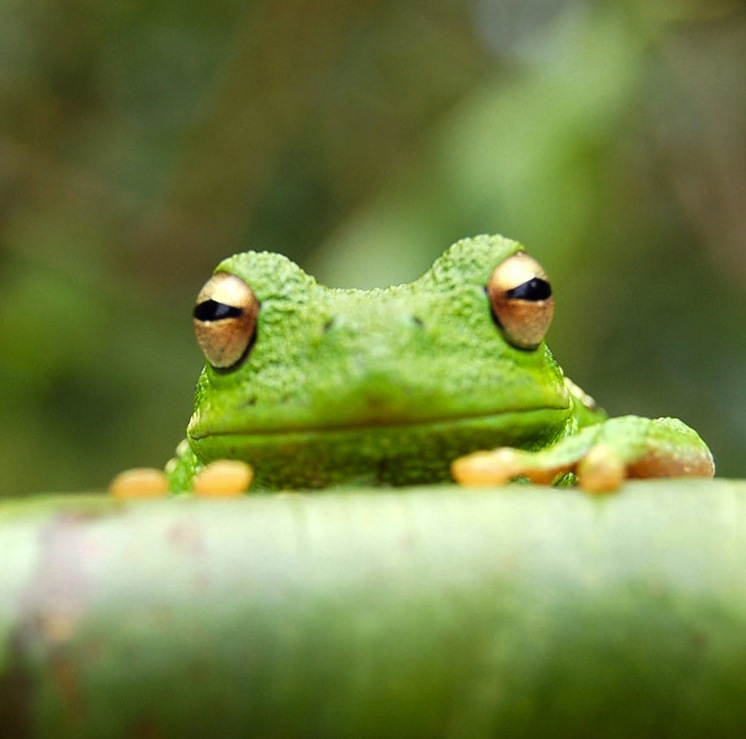
\includegraphics[width=0.5\textwidth]{frog.jpg}
\caption{\label{fig:frog}Лягушка}
\end{figure}
Пункты 1-7 отчета составляются строго до начала лабораторной работы. Допущен к выполнению работы.
\textbf{Подпись преподавателя}
\section{Распечатка протокола}
\section{Дневник отладки}
\begin{tabular}{|c|p{1cm}|p{1.5cm}|c|p{2.5cm}|p{2cm}|p{2.25cm}|}
    \hline
    № & Лаб. или дом. & Дата & Время & Событие & Примечание\\
    \hline
    1 & Дом. & 07.04.23 & 2:21 & Выполнение лабораторной работы & -\\
    \hline
\end{tabular}
\section{Замечания автора по существу работы}
\href{https://codeforces.com/contest/1798/submission/199301228}{Контест (Div. 2)}\\
\href{https://codeforces.com/contest/1798/submission/201243811}{Дорешка 1}\\
\href{https://codeforces.com/contest/1798/submission/201242217}{Дорешка 2}
\section{Выводы}
Были изучены и применены для оформления отчета лабораторной работы методы оформления документов в издательской системе \LaTeX.
\end{document}
